\documentclass[a4paper,11pt]{article}  
\pagestyle{plain}
\usepackage{siunitx, dirtytalk, hyperref, nicefrac, mathtools} 
\usepackage{graphicx,sectsty,longtable,tocloft,color,pdfpages,sidecap,subfig,array,eurosym}
 \captionsetup[figure]{labelfont={bf},name={Fig.},labelsep=period}

%\usepackage{refcheck} % places ??? for unused references in the PDF

\usepackage[english]{babel}
% smaller vertical spacing between references in bibliography
\let\OLDthebibliography\thebibliography
\renewcommand\thebibliography[1]{
  \OLDthebibliography{#1}
  \setlength{\parskip}{0pt}
  \setlength{\itemsep}{0pt plus 0.3ex}
}\usepackage{amsmath}
\usepackage{amsfonts}
\usepackage{amssymb}
%
% 2cm page margins (for A4)
%
\usepackage[left=2cm,right=2cm,top=2cm,bottom=2cm]{geometry}
\tolerance = 1000
\parindent 0cm
\parskip 2mm
%
% Section headings in Arial
%
\allsectionsfont{\sffamily}
%% Customise table of contents behaviour
\tocloftpagestyle{empty}
\renewcommand{\contentsname}{Table of Contents}
\renewcommand{\cfttoctitlefont}{\LARGE\bf\sffamily} 
% Add some width so section label A1.2.3.4 doesn't overlap with section title
\addtolength{\cftsecnumwidth}{3em}
\addtolength{\cftsubsecnumwidth}{3em}
\addtolength{\cftsubsubsecnumwidth}{3em}
%
% Some commonly used definitions
%
\def\urltilda{\kern -.15em\lower .7ex\hbox{\~{}}\kern .04em}
\def\urldot{\kern -.10em.\kern -.10em}
\def\urlhttp{http\kern -.10em\lower -.1ex\hbox{:}\kern -.12em\lower 0ex\hbox{/}\kern -.18em\lower 0ex\hbox{/}}
\def\xilinx{{\small\tt XILINX}}
\def\quarter{{$\frac{1}{4}$}}
\def\half{{$\frac{1}{2}$}}
\def\gm2{{\tt g-2}}
\def\geant{{\tt GEANT}}
\def\art{{\it art}}
\newcommand{\mue[1]}{{\tt Mu{#1}e}}
\newcommand{\gbp[1]}{\pounds\kern 0.08333em{#1}}
\newcommand{\eu[1]}{\euro\kern 0.08333em{#1}}
\newcommand{\usd[1]}{\$\kern 0.08333em{#1}}
%
\begin{document}
\pagenumbering{roman}
\thispagestyle{empty}
\begin{titlepage}
\begin{center}
	%\includegraphics[width=\textwidth]{fig/logo.png}
\end{center}
\begin{center}
	\vspace{1cm}
	{\huge \textbf{Tracker Alignment for the g-2 experiment:} \\ \textit{Summary of alignment results \\ with straight tracks.}}\\
	\vspace{1.5cm}

	\vspace{6cm}
	{\LARGE\bf Gleb Lukicov}\\
	{\Large University College London}
	\vspace{4cm}
	\vfill
	\vspace{0.9cm}
	{\large February 9, 2018}
\end{center}
\end{titlepage}
\clearpage

\pagenumbering{arabic}
\thispagestyle{plain}

\clearpage
\section{Introduction}
In order for the tracking detector to reduce the systematic uncertainty on the AMM measurement and improve the sensitivity to a muon EDM, the absolute position of the tracking modules must be know to better than \SI{50}{\micro\metre}. The hardware-level (i.e. survey) alignment allows one to set a precise position of the modules with respect to each other. However, individual straw effects such as reduced wire tension, can affect different straws in a different way. Therefore, a more precise physics-level (i.e. track-based) alignment, that considers such effects, is required. Track-based alignment will be implemented using real data from Run 0 using the \texttt{Millepede II} framework~\cite{mp2}. A Monte Carlo (MC) simulation will also be developed to understand the detector geometry and how this effects how well the alignment can be determined, as well as to test the alignment procedure itself. 

\section{Millepede II}
The alignment task can be summarised as a Least Squares Fit (LSF) problem with a very large number of parameters. In 3D space, there are 6 degrees of freedom: 3 for movement and 3 for rotation. If only the tracker station with 8 modules is considered, that results in 48 parameters for the fit. However, considering all 128 straws in each module increases this number to 6,144 parameters. In CMS, for example, a track-based alignment with 50,000 parameters was successfully implemented \cite{CMS} using the \texttt{Millepede II} package. 

The fitted parameters can be divided into two classes: global and local parameters. Global parameters (i.e. the alignment parameters) affect all tracks (e.g. position of a straw layer). Local parameters are associated with individual fitted tracks. For example, a straight line fit in 2D to a single track will have 2 local parameters: the slope and the intercept. \texttt{Millepede II} solves the linear LSF problem with a simultaneous fit of all global and local parameters minimising a function $F_j$, which is a function of a sum of residuals. A residual ($r_p$) is associated with a global parameter. We take a tracker straw layer here as an example. A residual is then given as the difference between the actual hit position ($y_i$) and the fitted (reconstructed) position in that layer $p$
\begin{equation}
r_p = y_i - f_i(\boldsymbol{p,q_j}),
\end{equation}
where $f_i(\boldsymbol{p,q_j})$ is fit parametrisation. And the $\chi^2$ of a distribution of residuals is given by
\begin{equation}
\chi^2 =\sum_{i=1}^{P}{\frac{(r_p)^2}{(\sigma_p^{\mathrm{det}})^2}},
\end{equation}
where $\sigma_p^{\mathrm{det}}$ is the detector resolution at layer $p$, and ($r_p$) is the residual in layer $p$. For the tracking detector, we are considering a constant detector resolution of \SI{150}{\micro\metre} \cite{g-2_TDR} for all straws. $F_j$ is minimised with respect to a variation of global ($\boldsymbol{p}$) and local ($\boldsymbol{q_j}$) parameters
\begin{equation}
F_j(\boldsymbol{p},\boldsymbol{q_j})=\frac{d\chi^2}{d(p_1, p_2,...,q_1, q_2)}=0.
\end{equation}
The phase space of the parameters is large, hence, the differential equation is first linearised and then reorganised into a block matrix equation \cite{mp2} for a sum over all tracks $j$ of the form
\begin{equation}
\left(\boldsymbol{C}\right)\left(\boldsymbol{d}\right) = - \left(\boldsymbol{g}\right),
\end{equation}
where $\boldsymbol{C}$ is a matrix containing the connection between local and global parameters, $\boldsymbol{d}$ is the correction vector (for global parameters), and $\boldsymbol{g}$ a vector of the normal equations~\cite{mp2}. Hence, a matrix inversion, whose dimension is given by the number of global parameters, is necessary to obtain the corrections to the global parameters that simultaneously minimises the $\chi^2$.

The user can write a Monte Carlo (MC) programme to: (1) fully describe the detector geometry (to understand its effects on the alignment), and (2) calculate the residuals for the fitted tracks, as well as to define the local and global parameters. A \texttt{C++} infrastructure (Mille) is provided to write these into a binary file which is passed to PEDE (a \texttt{Fortran} executable) which performs a simultaneous fit via a matrix inversion. The user is also responsible for writing a constraints file (specifying the redundant degrees of freedom), and a steering file (specifying the mathematical methods used by PEDE). The final output of the PEDE algorithm are labels and the corresponding fitted values of the global parameters (and their errors, if applicable). This procedure is shown in Fig.~\ref{fig:mp2}.
\begin{figure}[!ht]
	\centering
	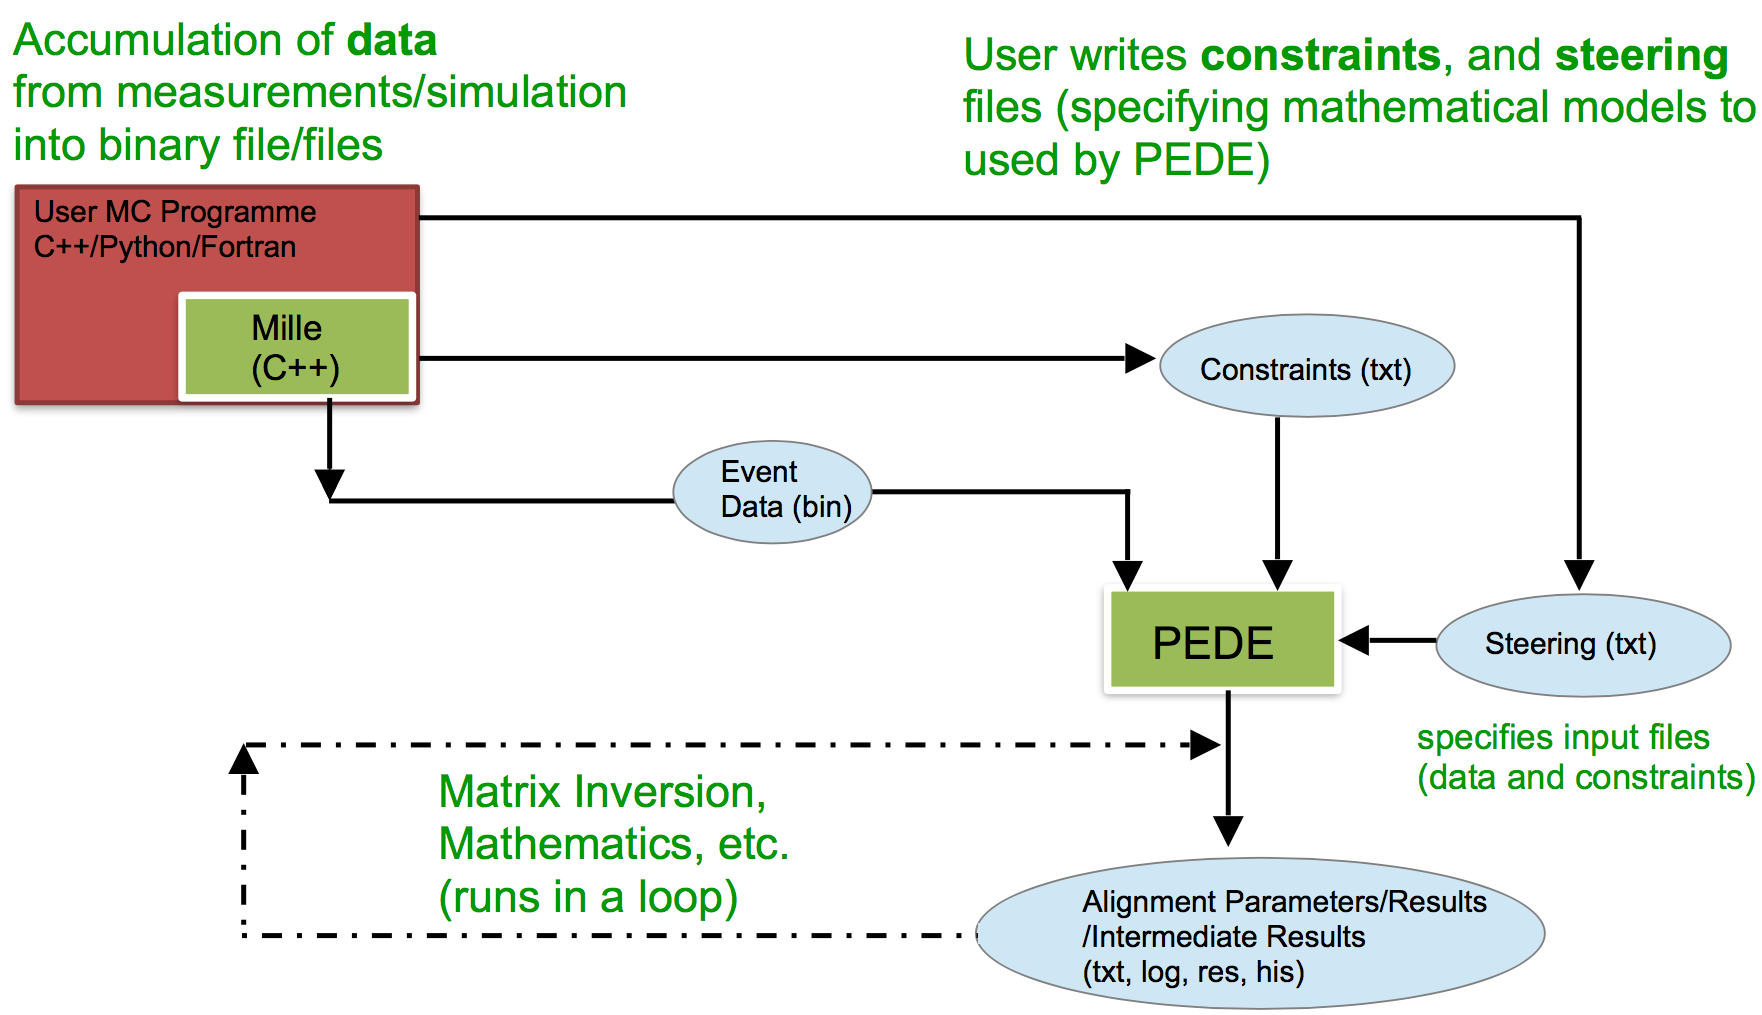
\includegraphics[scale = 0.4]{fig/MP2.png}
	\caption{The schematic of the \texttt{Millepede II} routine with the user MC programme. The MC code will be integrated with the g-2 \textit{art} offline analysis framework~\cite{art}, and the PEDE will be exported as a \texttt{Fortran} executable.}
	\label{fig:mp2}
\end{figure}
\vspace{-0.2cm}

To understand the \texttt{Millepede II} algorithm a translation (into \texttt{C++}) of the provided (\texttt{Fortran}) toy-model was implemented. The difference in results was consistent with within the precision of \text{C++} floating-point numbers ($10^{-7}$).
\vspace{-0.1cm}
\subsection{User MC Algorithm}
\vspace{-0.1cm}
An outline of the current MC code used to validate and test the alignment code using just four tracker modules, having 8 straws per layer (4 layers per module) with straight tracks in 2D is given below:
\vspace{-0.4cm}
\begin{enumerate}
	\setlength\itemsep{-0.5em}
	\item Define the ideal geometry (i.e. assumed straw coordinates).
	\item Define the misaligned geometry (i.e. actual (truth) straw coordinates due to misalignment, which is set in the MC).
	\item Generate straight ($y_{\rm{truth}} = m_{\rm{truth}}x+c_{\rm{truth}}$) tracks (through the misaligned geometry) 
	\item Calculate the Distance of Closest Approach (DCA) (see Fig.~\ref{fig:dca}) from the truth track and a straw in each layer.
	\item Smear the DCA by the detector resolution ($\sigma_p^{\mathrm{det}}$).
	\item Reconstruct the DCA in the ideal geometry.
	\item Fit a line ($y_{\rm{fit}} = m_{\rm{fit}}x+c_{\rm{fit}}$) to the reconstructed hit points (or reconstructed \textit{drift circles}, see Fig.~\ref{fig:drift}), and calculate the residual between the fit and the hit point.
	\item Pass residuals (as well as global and local parameters) to PEDE to allow for global minimisation of all residuals based on module movements using the matrix inversion method.
\end{enumerate}
\vspace{-0.1cm}
An example of five generated and reconstructed tracks in four tracker modules is shown in Fig.~\ref{fig:tracks}.
\clearpage
\begin{figure}[!ht]
	\centering
	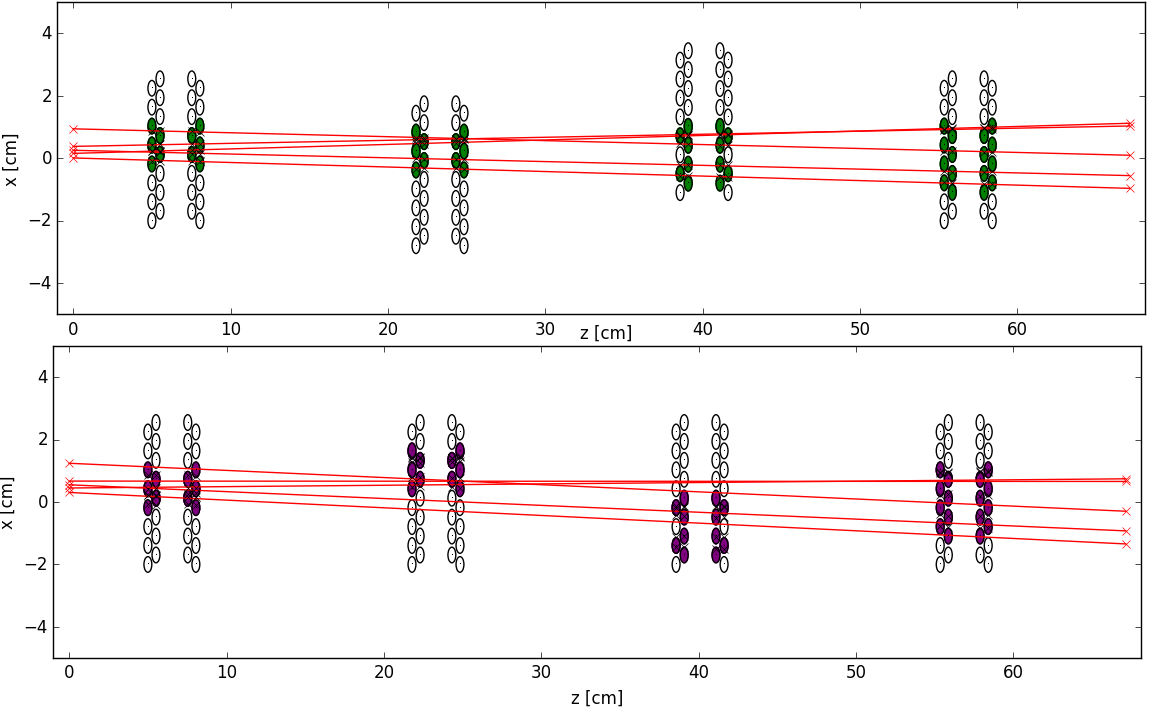
\includegraphics[scale = 0.43]{fig/tracks.png}
	\caption{Exaggerated effect of misalignment. \textbf{Top:} Simulated tracks through a misaligned tracker station. True hits in straws are shown in green. \textbf{Bottom:} Reconstructed tracks through the ideal geometry. The original truth hits are shown in purple.}
	\label{fig:tracks}
\end{figure}
The detected signal in the tracker comes from the collected charge on the central cathode wire in the straw. This charge is due to the ionisation electrons, liberated from Ar atoms by a charged particle traversing the straw. The liberated electrons drift towards the cathode wire, which is held at +1.6 kV. The absolute hit position in the straw is not know only a \textit{drift circle} (see Fig.~\ref{fig:drift}), a radius of which is given by the DCA. The track trajectory is then reconstructed from multiple straws via extrapolation to all modules via a \textit{circle fit}. 
\begin{figure}[!ht]
\centering
\subfloat[]{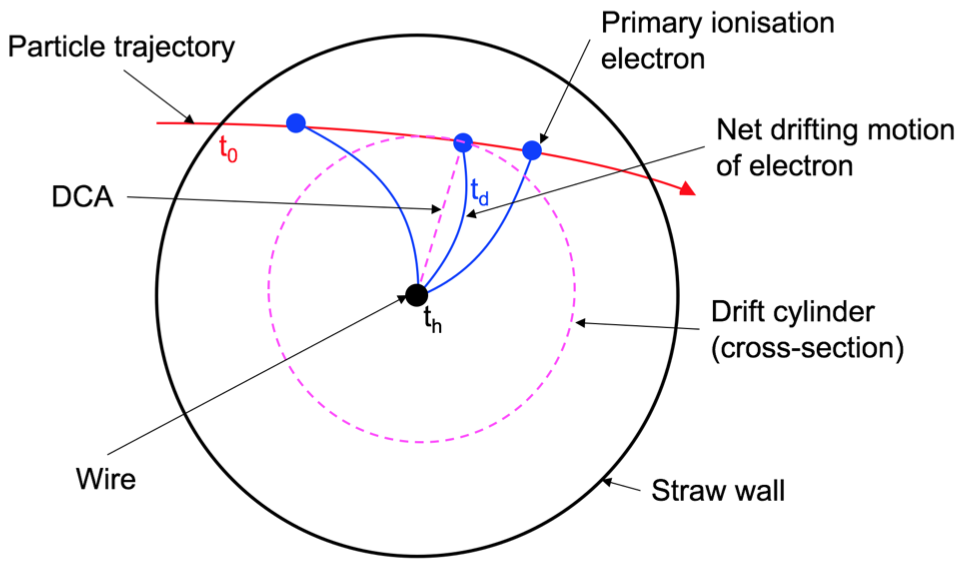
\includegraphics[scale = 0.26]{fig/dca_Tom.png}}
\subfloat[]{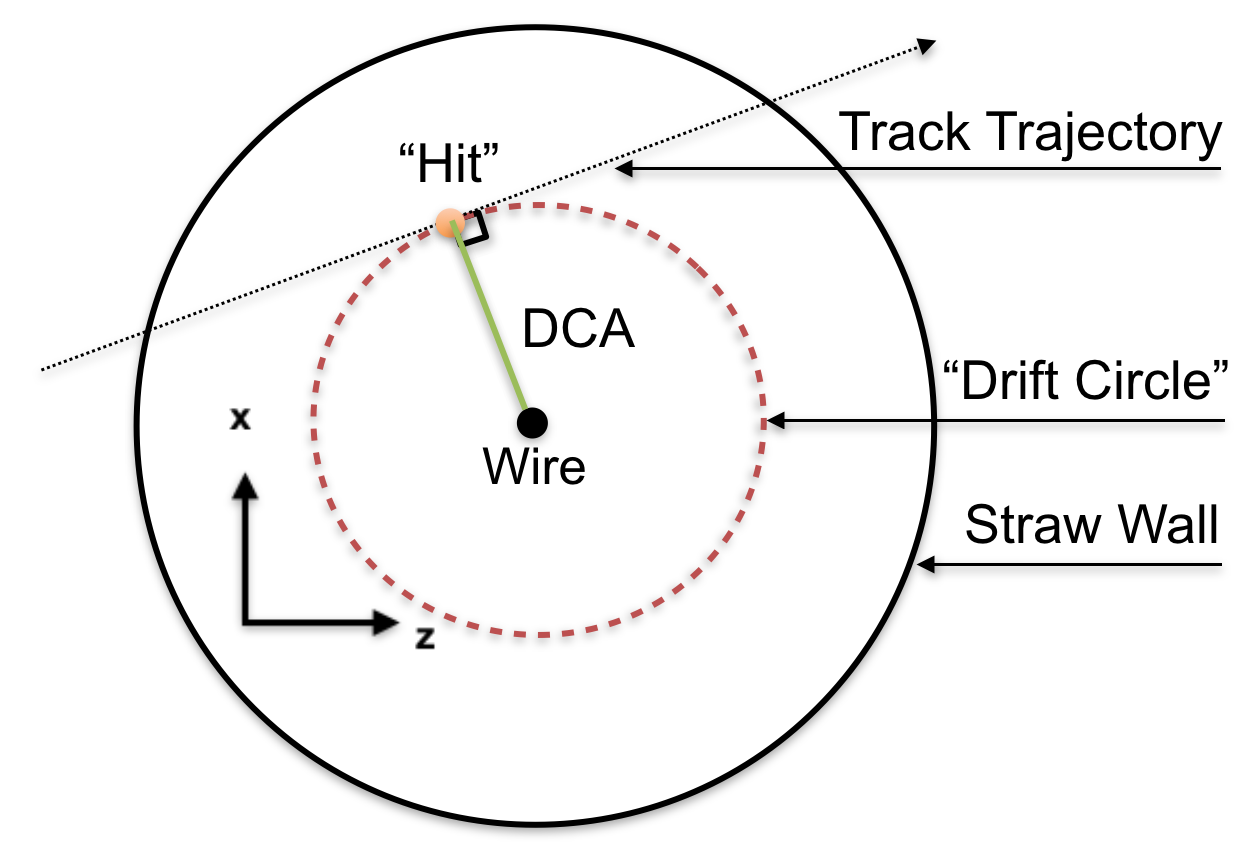
\includegraphics[scale = 0.17]{fig/dca.png}}
    \caption{ a) Diagram of the relationship between the drifting of primary ionisation electrons to the straw wire and the DCA reconstructed from the time taken by this drift. The drift circle specified by the DCA is also shown~\cite{Tom}. Diagram courtesy of Tom Stuttard. b) DCA calculation in the MC simulation for straight tracks with no magnetic field.}
\label{fig:dca} 
\end{figure}
\section{The Alignment Overview: 1D case.}
First of all, I have considered a 1D misalignment with the first and the last modules \textit{fixed}. This means that there is no misalignment to these modules, additionally, this corresponds to a constraint of 1.0 for the global label for this module in PEDE. It is essential to define the four distinct manifestations of misalignment:

1) $M^{c}_p$ is the \textit{characteristic} misalignment, which is specific for each individual layer $p$. $M^{c}_p$ is either set in the simulation, or estimated in PEDE as the final parameter. \\
2) $M_0$ is the \textit{overall} misalignment given by
\begin{equation}
M_0 = \frac{\sum_{i=1}^{P} M_i}{P},
\end{equation}
where $P$ is the total number of the detector layers.\\
3) $M^r_p$ is the \textit{relative} misalignment per layer, which is given by
\begin{equation}
M^r_p=M^{c}_p-M_0.
\end{equation}
4) $M^{s}_p$ is the \textit{shear} misalignment and corresponds to the mean of the residual ($\langle r_p \rangle$) for layer $p$
\begin{equation}
M^{s}_p = \langle r_p \rangle =  M^{c}_p  - M_0 - \frac{z_p\cdot \sum_{i=1}^{P}{ M^{c}_i \cdot z_i}}{\sum_{i=1}^{P}{z_i^2}},
\label{eq:shear}
\end{equation}
where $z$ is the horizontal position (along the beam) of a layer. It is also necessary to introduce two variables that characterise the fitted track.
The $\langle r_p \rangle$ for a 1D displacement is given by
\begin{equation}
\langle r_p \rangle = \frac{\sum_{j=1}^{N}{r_{j,p}}}{N},
\end{equation}
where $N$ is the total number of tracks, while the standard deviation (SD) for a distribution of residuals at layer $p$ is given by
\begin{equation}
\sigma_p = \frac{\sum_{j=1}^{N}{r_{j,p} - \langle r_p \rangle}}{N}.
\end{equation}
Using the above equations, it is possible to show that the expected mean $\chi^2$ for a given set of characteristic misalignments is given by
\begin{equation}
\langle \chi^2_{\rm{Mis}} \rangle = N - 2 +  \frac{
	\sum_{i=1}^{P}(M^{s}_i)^2-\frac{\sum_{i=1}^{P}{(M^{s}_i)^2}}{P} - 
	\frac{2 \cdot \sum_{i=1}^{P}M^{s}_i \cdot z_i}{\sum_{i=1}^{P}(z_i)^2}}
{\sum_{i=1}^{P}(\sigma_p^{\mathrm{det}})^2},
\label{eq:chi2}
\end{equation}
where the summation is over all layers. The misalignment for a straight track shifts the mean of the residuals for the misaligned and the non-misaligned modules (hence it was defined as the \textit{shear} misalignment, $M^{s}_p$). Moreover, the expected SD of residuals at layer $p$ is given by
\begin{equation}
\sigma_r=\sigma\sqrt{\frac{P-1}{P}-\frac{z_i^2}{\sum_{i=1}^{P} z_i^2}}.
\label{eq:res}
\end{equation}

\subsection{Comparison of MC Results with Analytical Predictions}
The derived equations for $\langle \chi^2_{\rm{Mis}} \rangle$, $\sigma_r$ and $M^{s}_p$ must be tested over a range of misalignment scenarios to test the validity of the alignment procedure in order to better understand the detector geometry and its effect on the track-fitting. Results for an asymmetric misalignment case with module 1 and 2 misaligned by \SI{500}{\micro\metre} and \SI{1000}{\micro\metre}, respectively, is given in Fig.~\ref{fig:res} and Fig.~\ref{fig:chi2}. Finally, a comparison between the input misalignment from the MC simulation and the final result produced by PEDE was performed as a function of the number of fitted tracks as shown in Fig.~\ref{fig:pede}. The non-fixed modules 1 and 2 display acceptable differences above 5,000 tracks.
\clearpage
\begin{figure}[!ht]
	\centering
	\subfloat[]{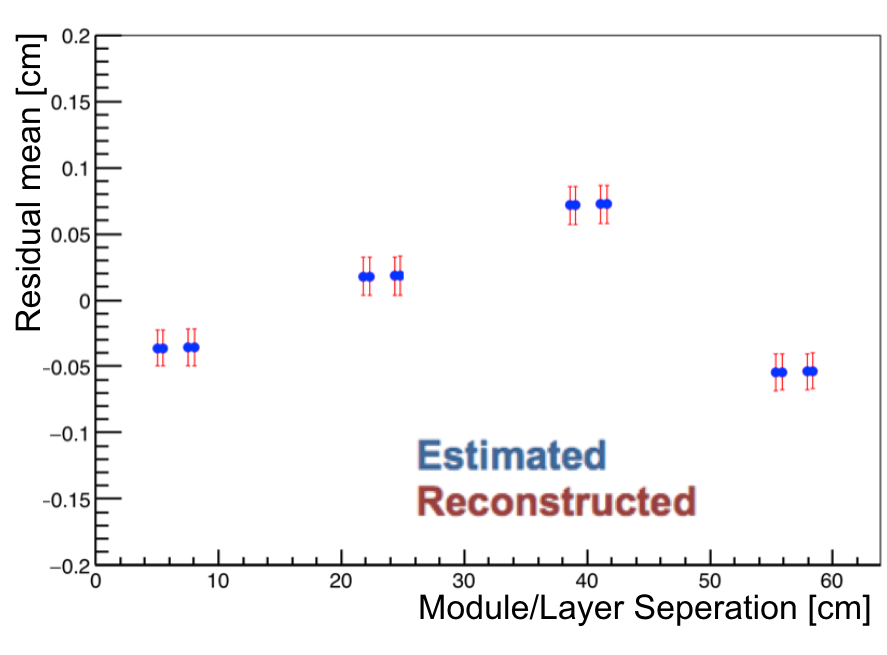
\includegraphics[scale = 0.265]{fig/shear.png}}
	\subfloat[]{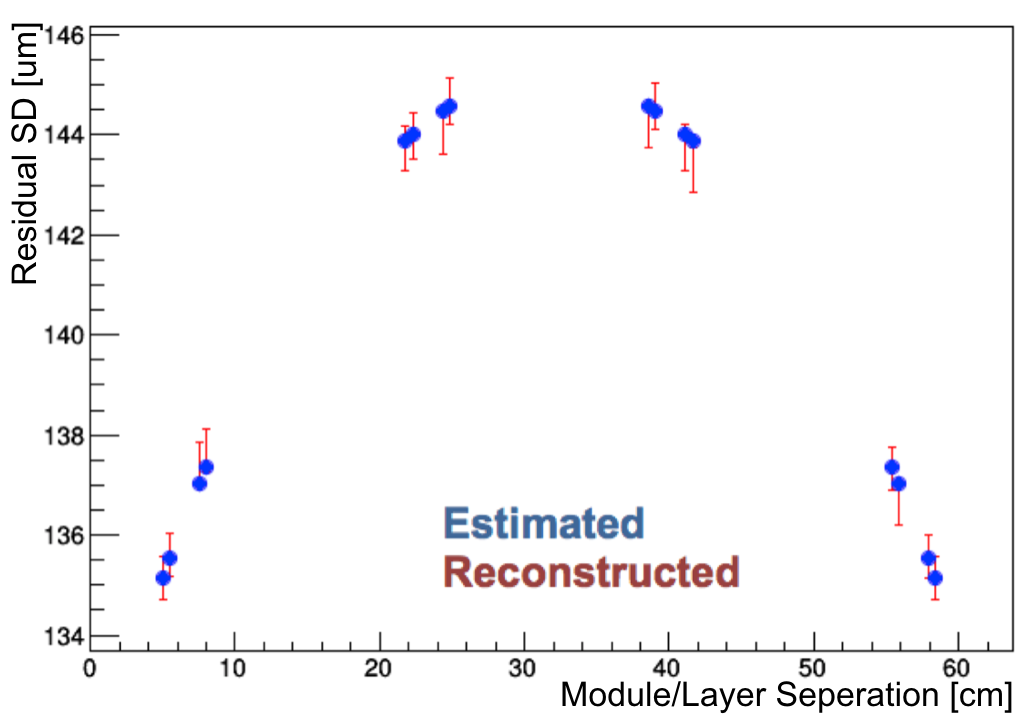
\includegraphics[scale = 0.235]{fig/res.png}}
	\vspace{-0.15cm}
	\caption{Prediction (in blue) and reconstructed (in red) alignment parameters with 50,000 tracks: a) The net effect of the misalignment shifts the mean position of the residuals in each layer according to Eq.~\ref{eq:shear}. b) The resolution SD is smaller on the outer modules (M0 and M3) as seen in Eq.~\ref{eq:res}. This can be conceptually understood as the ability for a better fit away from the mean vertical ($z$) position, as the best fit line always passes through the mean $z$. Hence, a change in the gradient will have a larger effect for the outer modules. }
	\label{fig:res}
\end{figure}
\vspace{-0.1cm}
\begin{figure}[!ht]
	\centering
	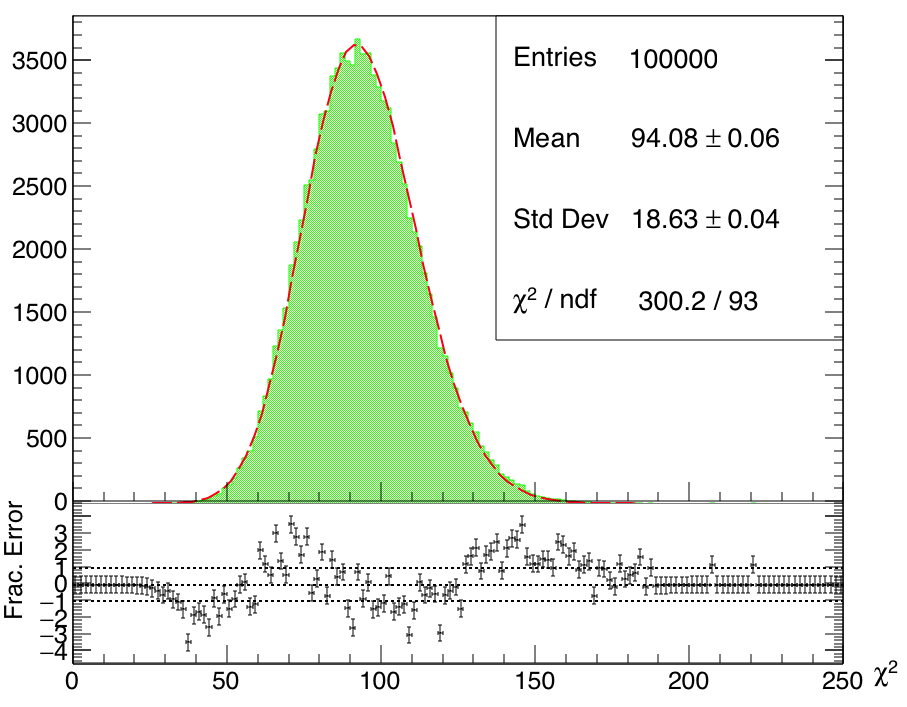
\includegraphics[scale = 0.26]{fig/chi2.png}
	\vspace{-0.1cm}
	\caption{$\chi^2$ distribution from the MC simulation (in green), and fit (in red) with expected $\langle \chi^2_{\rm{Mis}} \rangle$ = 94.04, as predicted by Eq.~\ref{eq:chi2}. The fractional error shows how many SD the fit function differs from the simulation data: $\frac{\chi^2_{\rm{data}}-\chi^2_{\rm{fit}}}{\sigma_{\chi^2_{\rm{data}}}}.$} \label{fig:chi2}
\end{figure}
\vspace{-0.35cm} 

\clearpage
\begin{figure}[!ht]
	\centering
	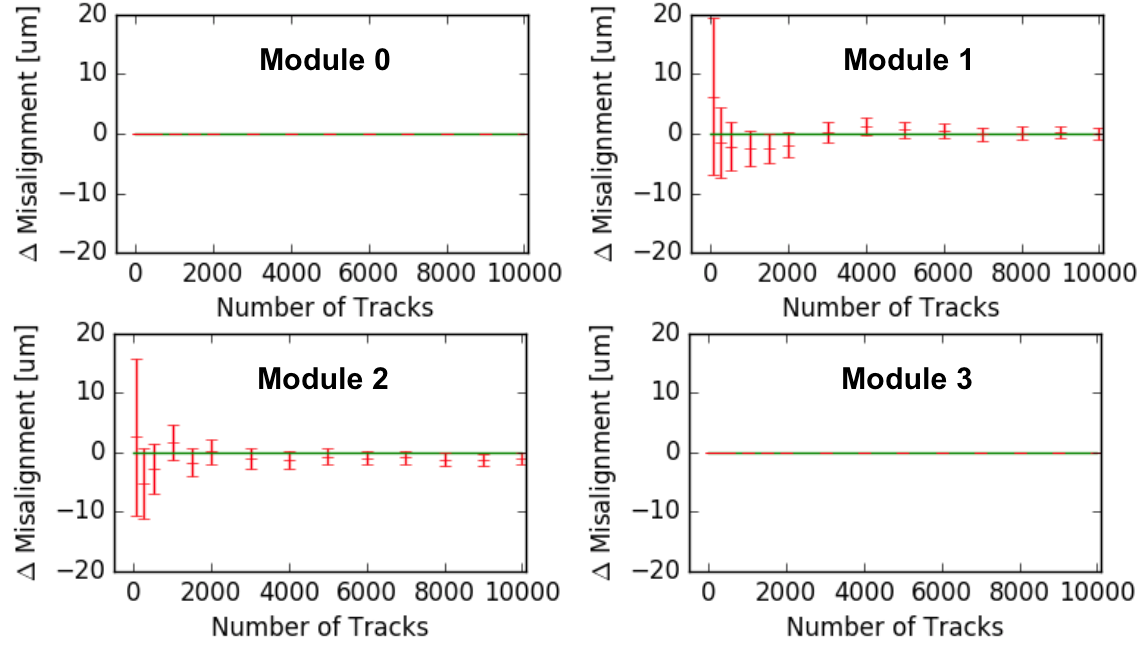
\includegraphics[scale = 0.33]{fig/PEDE.png}
	\vspace{-0.3cm}
	\caption{Figure of Merit: The difference in misalignment 
		between the simulation input and the PEDE 
		prediction vs. the number of generated tracks. The inversion method (which gives an estimate on the error) with 1 iteration and convergence ($\Delta \boldsymbol{F}$) interval of 0.01 was used in the PEDE steering file.}
	\label{fig:pede}
\end{figure}
\vspace{-0.6cm}
\begin{figure}[!ht]
\centering
\subfloat[]{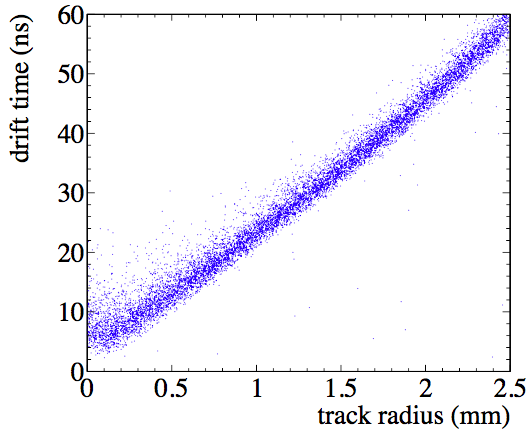
\includegraphics[scale = 0.36]{fig/drift.png}}
\subfloat[]{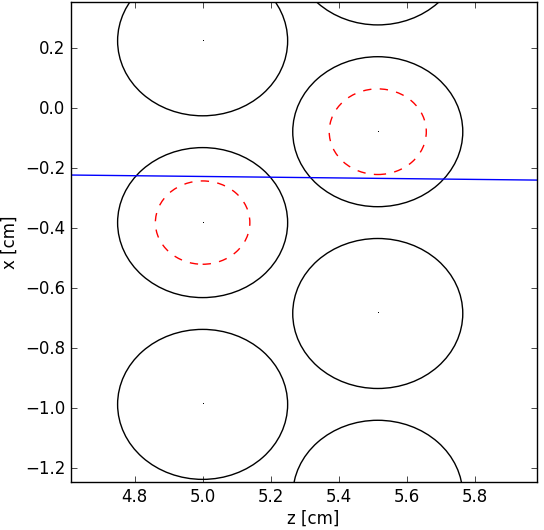
\includegraphics[scale = 0.40]{fig/circles.png}}
    \vspace{-0.1cm}
    \caption{a) Time versus distance relation in a single straw predicted by \texttt{GARFIELD}~\cite{GARFIELD} simulation for 50:50 Ar:Ethane at a gain of $10^6$ for a 1.5 T magnetic field~\cite{g-2_TDR}. b) Truth hit drift circles (smeared) in a single module.}
\label{fig:drift} 
\end{figure}
\vspace{-0.4cm}

\section{2D Misalignment with circle-fit.}
\vspace{-0.2cm}
After that, a MC framework with 2D misalignment (with rotations) with \textit{circle fit} was implemented. This is done to match the reconstruction of the real data, where only the hit times are known, from which, given a know drift velocity (see Fig.~\ref{fig:drift}), a distance (i.e. the radius of the drift circle) can be reconstructed. The ambiguity in the trajectory is resolved by combining two drift circles to form a doublet, and the 2D hit position is resolved by combining two doublets. Multiples 2D position from many modules give a 3D track. Due to the empirical nature of the circle-fit (which is performed by finding the minima algebraically) the exact analytical predictions for $\sigma_r$, and $\langle \chi^2_{\rm{Mis}} \rangle$ cannot be derived. However, other tools exist to check the solutions, as will be described in the next sections.

\subsection{2D Misalignment in x and z via a generic rotations.}

The aim of this section is to evaluate circle-fit residuals ($R$) with misalignment ($M$) as an anti-clockwise (AC) rotation ($\theta$) along the beam axis ($z=0$) through the detector centre. We now have 3 coordinate systems to refer to the straw positions (see Fig.~\ref{fig:theta}): \\
1) global coordinates ($z$, $x$) - relative to the \say{global} (0, 0). The derivatives of interest should be given w.r.t these coordinates. \\ 
2) local (\say{detector}) coordinates ($z_d$, $x_d$) in the \say{un-rotated} frame - relative to the centre of rotation of a detector, which is given by ($z^{centre}$, $x^{centre}$). These are orthogonal to the global coordinates. \\ 
3) local (\say{detector}) coordinates ($z'_{d}$, $x'_d$) in the rotated frame. Such that, for a centre of rotation ($z^{centre}_d$, $x^{centre}_d$) = ($z^{',centre}_{d}$, $x^{',centre}_d$) = (0,0), in the local coordinates.
\begin{figure}[!ht]
\centering
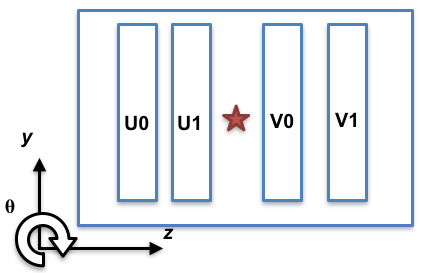
\includegraphics[width=0.9\linewidth]{fig/theta.png}
\caption{The definition of the 3 coordinate systems.}
\label{fig:theta}
\end{figure}\\
With $z_d'=z_d(\theta)$ and $x'_d=x_d(\theta)$ transformations (the action of AC rotation) is given by
\begin{equation}
\begin{bmatrix}z_d'\\x_d'\\\end{bmatrix}=\begin{bmatrix}\cos \theta &-\sin \theta \\\sin \theta &\cos \theta \\\end{bmatrix} \begin{bmatrix}z_d\\x_d\\\end{bmatrix} = \begin{bmatrix}z_d\cos \theta -x_d\sin \theta \\z_d\sin \theta +x_d\cos \theta \\\end{bmatrix}.
\end{equation}
Then, we need to translate back to the global coordinates by
\begin{equation}
\begin{bmatrix}z\\x\\\end{bmatrix}=\begin{bmatrix}z_d'+z^{centre}\\x_d'+x^{centre}\\\end{bmatrix}=\begin{bmatrix}z_d\cos \theta -x_d\sin \theta + z^{centre} \\z_d\sin \theta +x_d\cos \theta + x^{centre} \\\end{bmatrix}. \label{eq:global}
\end{equation}
In the end, we need an expression for $\frac{\partial R}{\partial\theta}$ in terms of \textbf{reconstructed} (i.e. measured) parameters only. Essentially, 
\begin{equation}
\frac{\partial R}{\partial\theta} = \frac{\partial DCA(z,x,m,c)}{\partial\theta}= \frac{\partial DCA(z(\theta),x(\theta),m,c)}{\partial\theta},
\end{equation}
or, more generally, 
\begin{equation}
\frac{\partial R}{\partial\theta} = \frac{\partial R}{\partial m}\frac{\partial m}{\partial \theta} == \frac{\partial DCA(\theta)}{\partial\theta} = \frac{\partial DCA(m)}{\partial m}\frac{\partial m(\theta)}{\partial \theta},  \label{eq:partialRM}
\end{equation}
where $m$ represents a measurement (e.g. straw displacement in $z$ or $x$).
We can now write the equation for a residual (defined in Fig.~\ref{fig:resPic}) using Eq.~\ref{eq:global}
\begin{equation}
\begin{split}
\mathrm{Residual}= R =\mathrm{Point \ To \ Line \ DCA} - \mathrm{Drift \ Circle \ Radius} = DCA(z(\theta),x(\theta),m,c) - r = \\
= \frac{ |c+mz(\theta)-x(\theta)| }  { \sqrt{m^2+1} } -r = \frac{ |c+m(z_d\cos \theta -x_d\sin \theta + z^{centre})-(z_d\sin \theta +x_d\cos \theta + x^{centre})| }  { \sqrt{m^2+1} } -r=\\ = \frac{ |c+mz_d\cos \theta -mx_d\sin \theta + mz^{centre} -z_d\sin \theta - x_d\cos \theta - x^{centre}| }  { \sqrt{m^2+1} } -r.
\end{split}
\end{equation}
\clearpage
\begin{figure}[!ht]
\centering
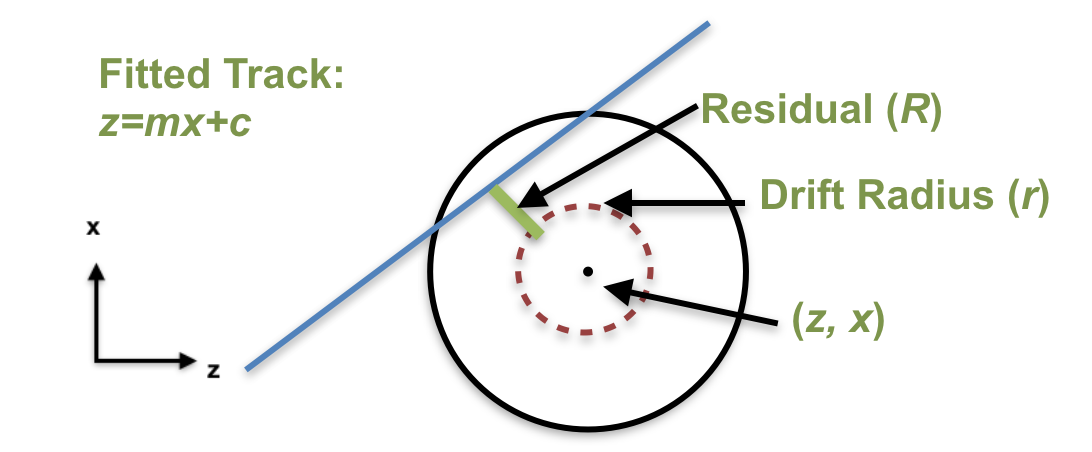
\includegraphics[width=0.6\linewidth]{fig/resPic.png}
\caption{The pictorial representation of a residual.}
\label{fig:resPic}
\end{figure}
We can now use Eq.~\ref{eq:partialRM} to write the expression for the desired residual expressed without the use of truth parameters (i.e. $\theta$)
\begin{equation}
\begin{split}
\frac{\partial R}{\partial\theta} = \frac{\partial R}{\partial z}\frac{\partial z}{\partial \theta} + \frac{\partial R}{\partial x}\frac{\partial x}{\partial \theta} = \\ \frac{ m(c+mz-x) }  { \sqrt{m^2+1} \cdot |c+mz-x| } \times (-z_d\sin \theta - x_d\cos \theta) \ + \\ \frac{ c+mz-x }  { \sqrt{m^2+1} \cdot |c+mz-x| } \times (z_d\cos \theta - x_d\sin \theta) = \\
\frac{ m(c+mz-x) }  { \sqrt{m^2+1} \cdot |c+mz-x| } \times (-x'_d) + \\ \frac{ c+mz-x }  { \sqrt{m^2+1} \cdot |c+mz-x| } \times (z'_d) = \\
\frac{ m(c+mz-x) }  { \sqrt{m^2+1} \cdot |c+mz-x| } \times (-x + x^{centre}) + \\ \frac{ c+mz-x }  { \sqrt{m^2+1} \cdot |c+mz-x| } \times (z - z^{centre}).
\end{split}
\end{equation}
where all inputs come either from measurement or assumption of ideal geometry (i.e. no truth inputs).
The full set of inputs to PEDE from a circle-fit with misalignment ($M$) as an anti-clockwise (AC) rotation ($\theta$) along the beam axis ($z=0$) through the detector centre, as well as all other cases of misalignment, is presented in Sc.~\ref{sec:deriv}.

\clearpage
\subsection{Results from MC and PEDE.}
The effect of misalignment affects the truth geometry of the detector, and not the reconstructed magnitude of the DCA, which is unchanged by the misalignment. This is justified, as we get a defined drift time irrespective of a global position of a straw. 

At the point of generation of a hit, the hit is assigned Left or Right (LR) \say{sign}. For example, if the his is generated on the left side of the straw centre relative to the beam, it will be an \say{L} hit. Hits generated close to the straw centre can be smeared to the other side, biasing the fit if the truth LR information is used. This effect can be further magnified if the said hit is further misaligned in the same direction (i.e. away from the truth hit position) by the effect of misalignment. For this reason, a cut on tracks with any hits less than \SI{500}{\micro\metre} is implemented, if LR truth information is used in the circle fit. 

A distribution of p-values of reconstructed tracks for a case of no misalignment and with module 3 misaligned by - \SI{20}{\micro\metre} in $x$, \SI{10}{\micro\metre} in z and rotated through the module centre by $0.3^{\circ}$ is shown in Fig.~\ref{fig:pval}.
\vspace{-0.2cm}
\begin{figure}[!ht]
\centering
\subfloat[]{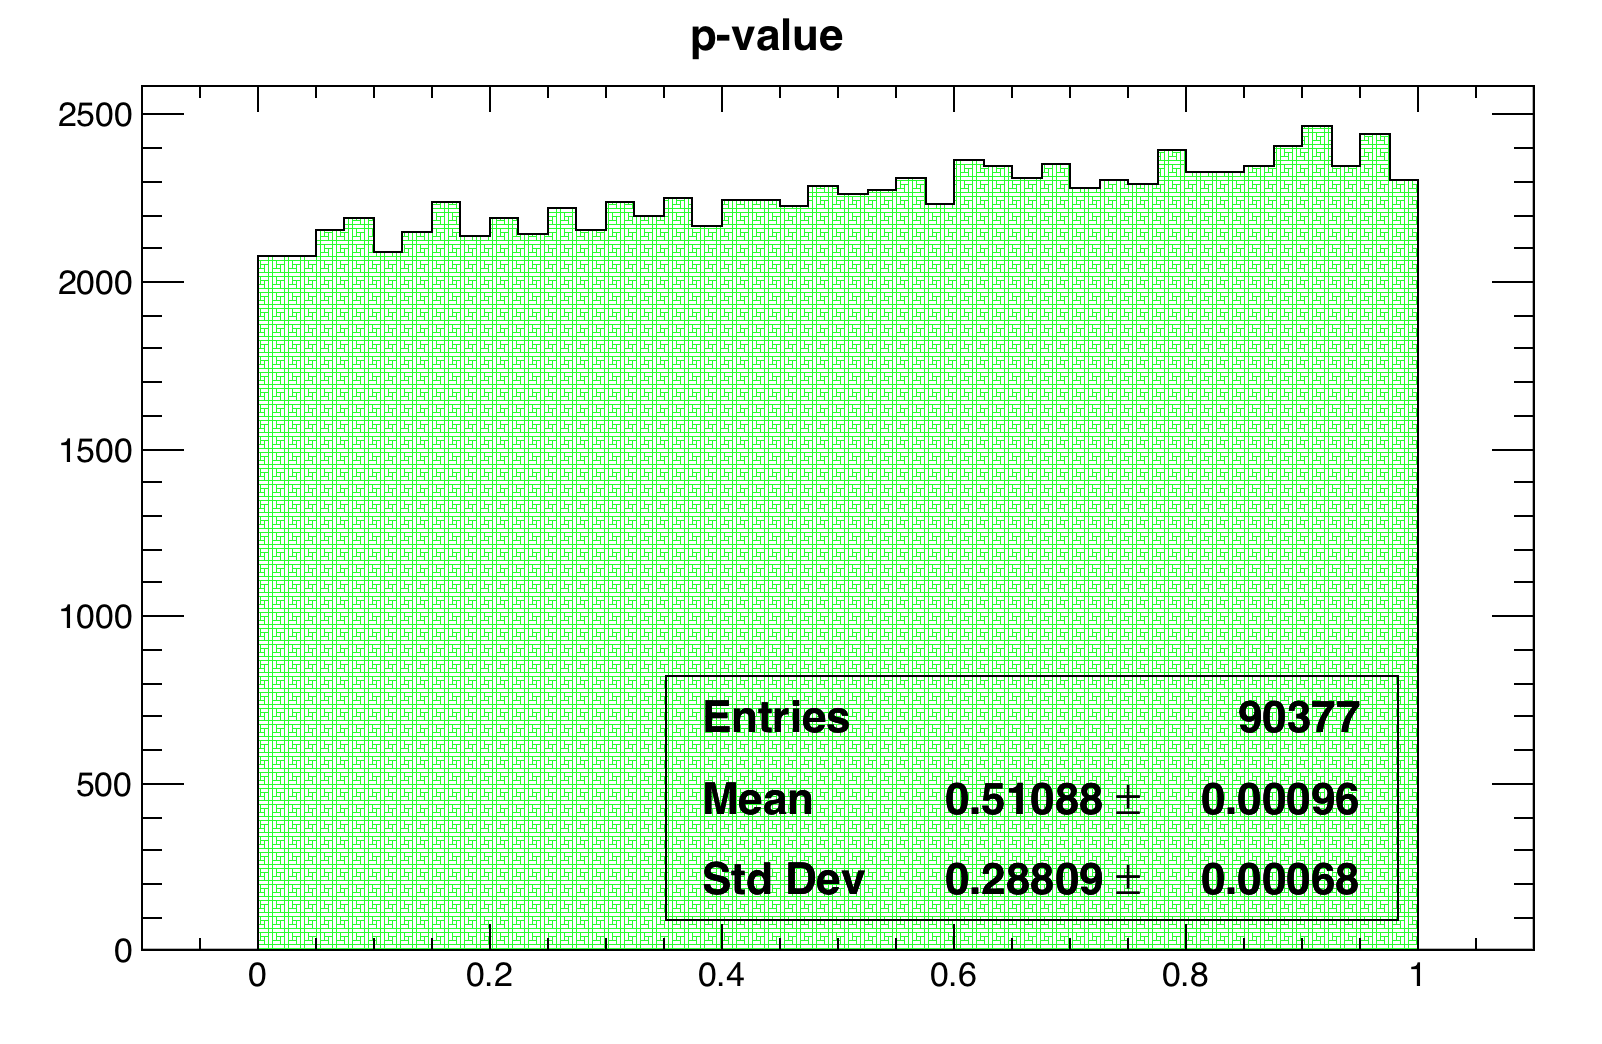
\includegraphics[scale = 0.3]{fig/p1.png}}
\subfloat[]{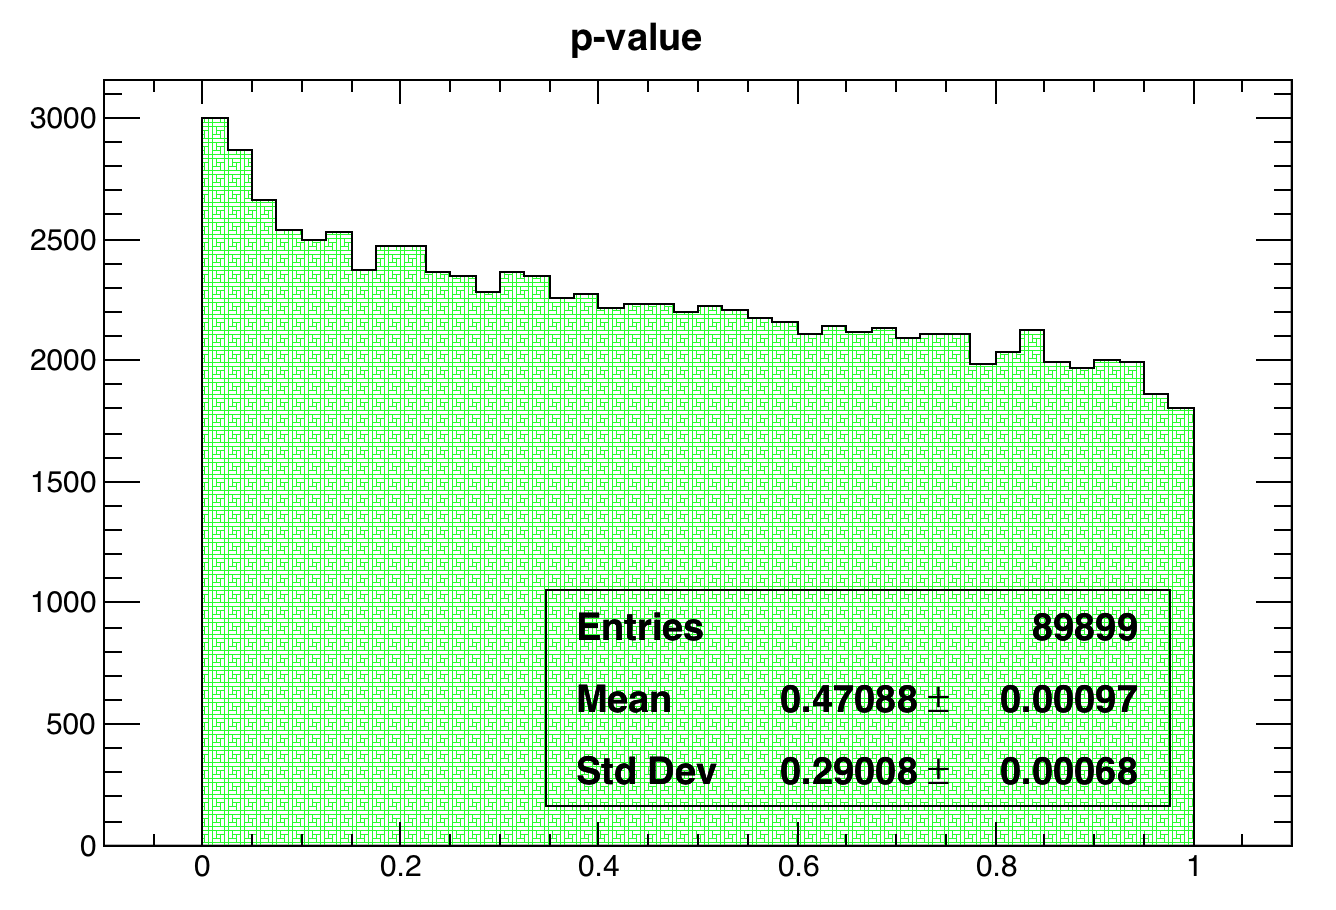
\includegraphics[scale = 0.34]{fig/p2.png}}
    \vspace{-0.1cm}
    \caption{Distribution of p-values for 1M requested tracks. The DCA ($\leq$ \SI{500}{\micro\metre}) rejection on tracks eliminated 90\% of tracks, which introduces a small bias. a) No misalignment b) Module 3 is misaligned, with increased residuals contributing small p-values.}
\label{fig:pval} 
\end{figure}
\vspace{-0.2cm}\\
Finally, a figure-of-merit for alignment capability of pede for misaligned modules 2 and 3 in $x$, $z$ and $\theta$ is shown in Fig.~\ref{fig:PEDEFOM}.
\vspace{-0.2cm}
\begin{figure}[!ht]
\centering
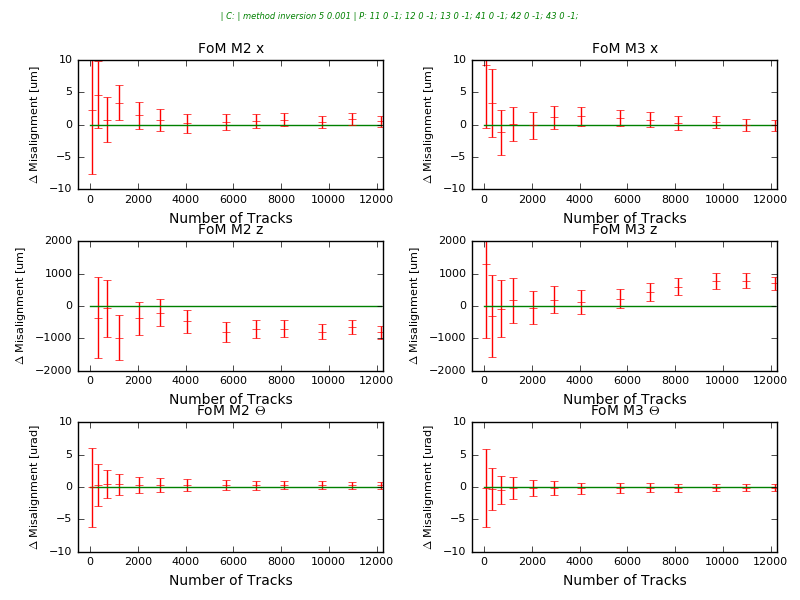
\includegraphics[scale = 0.45]{fig/pedefom.png}  
    \vspace{-0.1cm}
    \caption{Figure of Merit: The difference in misalignment between the simulation input and the PEDE prediction vs. the number of generated tracks.}
\label{fig:PEDEFOM} 
\end{figure}
\vspace{-0.2cm}

\clearpage

\section{3D Geometry.}\label{sec:3D}

In this section we will consider a case of misalignment in 3D, with tracker geometry coming from \textit{art}. The residual of interest, between the reconstructed track through the detector and the \say{drift cylinder}, is now a function of DCA between two skew lines. The assumption of the two lines (track and straw wire) being non-parallel will hold for all physical tracks of interest; the track and the wire can intersect, however. The definition of the initial (global) coordinate system is given below in Fig.~\ref{fig:4M}. \\
\vspace{-0.2cm}
\begin{figure}[!ht]
\centering
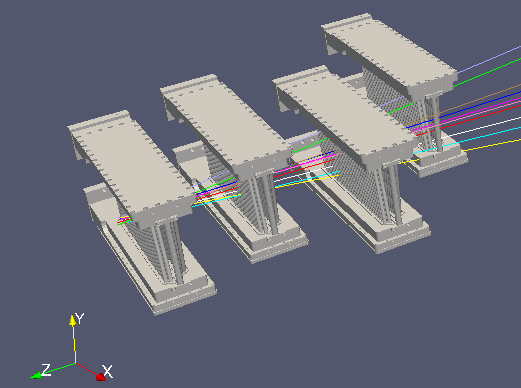
\includegraphics[scale = 0.45]{fig/4M.png}  
    \vspace{-0.1cm}
    \caption{Straight MC truth tracks through a misaligned station (in $x$) of 4 tracker modules.}
\label{fig:4M} 
\end{figure}
\vspace{-0.2cm}
First of all, consider parametrisation of the track. The slope of a line in $i$ direction is given by
\begin{equation}
m_i = \frac{p_i}{|\bf{p}|}, 	
\end{equation}
where $p_i$ is the momentum in $i$ direction, and $\textbf{p}$ is the momentum vector. 

A line in 3D can be parametrised with a variable parameter $t$ as follows
\begin{equation}
\textbf{r}(t) = \begin{pmatrix}x_L + m_x  t\\y_L + m_y t\\z_L + m_z t\\\end{pmatrix},
\end{equation}
where ($x_L, y_L, z_L$)  is some point on the line. However, we only need 4 parameters, out of 6 defined above, to specify the line. A 3D line is defined by two points, each with 3 DoF, giving 6 DoF for the line. The line, however, is invariant under the translation of either of the points along the line, giving 4 DoF. Assuming the track is not parallel to the $xy$ plane, as will be the case for all tracks of interest here, we can remove $z_L$, and $m_z$ dependence, by setting $z_0=0$, and dividing by $m_z$. 
\begin{equation}
\textbf{r}_T(t) = \begin{pmatrix}x\\y\\z\\\end{pmatrix} = \begin{pmatrix}x_L + \frac{p_x}{p_z}  t\\y_L + \frac{p_y}{p_z}  t\\  t\\\end{pmatrix} = \begin{pmatrix}x_L + p_x^{'} t\\y_L + p_y^{'}  t\\  t\\\end{pmatrix}= \textbf{v}t+\textbf{r}_T^0=\begin{pmatrix}p_x\\ p_y \\  1\\\end{pmatrix}t + \begin{pmatrix}x_L \\y_L  \\  0\\\end{pmatrix},
\label{eq:track}
\end{equation}
in the future, we will drop the $^{'}$ notation on momentum components. Therefore, we have decided to
parametrise our track with the following local parameters $\textbf{b}$
\begin{equation}
\textbf{b} = \begin{pmatrix}x_L \\y_L \\p_x \\ p_y\end{pmatrix}
\end{equation}


\subsection{Track to Wire distance with 3 DoF.}

First of all, we will consider a simpler case with 3 DoF on the detector component - the straw wire. The global alignment parameters $\textbf{a}$ are
\begin{equation}
\textbf{a} = \begin{pmatrix}x_W \\z_W \\m_x \end{pmatrix},
\end{equation}
which correspond to the displacements in $x$, $z$, as well as a rotation in the $xy$ plane. 

Now we are ready to tackle the real residuals, with DCA between the track and the wire given by
\begin{equation}
DCA = || \textbf{W} - \textbf{T} || = || \begin{pmatrix}x'_W - x'_T\\y'_W - y'_T\\z'_W - z'_T\\\end{pmatrix} || = \sqrt{ (x'_W - x'_T)^2 + (y'_W - y'_T)^2 + (z'_W - z'_T)^2},
\end{equation}
where \textbf{W} and \textbf{T} are the points of closest approach between the wire and the track, respectively - as indicated by the $'$ notation on the coordinates. With vector $\bf{WT}$ perpendicular to both the wire and the track. In order to form the required derivatives w.r.t local and global parameters, we need a functional form of DCA expressed in terms of the reconstructed track parameters and the wire parameters.
\begin{figure}[!ht]
\centering
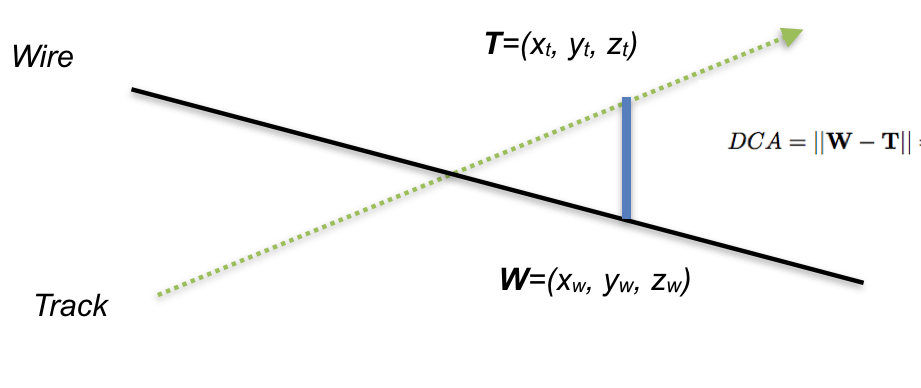
\includegraphics[width=0.6\linewidth]{fig/WireLine.png}
\caption{Track to wire DCA.}
\label{fig:WireLine}
\end{figure}

The wire can be parametrised as 
\begin{equation}
\textbf{r}_W(s) = \begin{pmatrix}x\\y\\z\\\end{pmatrix} = \begin{pmatrix}x_W + m_x s\\ s\\  z_W\\\end{pmatrix} = \textbf{u}s+\textbf{r}_W^0=\begin{pmatrix} m_x \\ 1\\  0\\\end{pmatrix}s + \begin{pmatrix}x_W  \\0 \\  z_W\\\end{pmatrix},
\label{eq:wire}
\end{equation}
as the position on the straw is constant with $z$, and slope in $x$ is due to the \textit{stereo angle} of $\sim 7.5^{\circ}$, the straw wire is in fact parallel to the $xy$ plane. Additional wire parameters can be added later (e.g. rotation in the $zx$ plane).

Here, we take a geometrical approach to express the above requirements on the DCA as
\begin{equation}
DCA = |\frac{\textbf{u} \times \textbf{v} \cdot (r^0_W - r^0_T) }{||\textbf{u} \times \textbf{v}||}| = ||\textbf{n}|| \cdot |(r^0_W - r^0_T)| ,
\end{equation}
which projects the distance between the \say{intercepts of the lines} (or any other points), to the normal between the two lines. Using the parametrisations defined above
\begin{equation}
\begin{split}
DCA(x_T, y_T, p_x, p_y, x_W, z_W, m_x) = \frac{|\begin{pmatrix} m_x \\ 1\\  0\\\end{pmatrix} \times \begin{pmatrix} p_x\\ p_y \\  1\\\end{pmatrix} \cdot (\begin{pmatrix}x_W  \\0 \\  z_W\\\end{pmatrix} - \begin{pmatrix}x_T \\y_T  \\  0\\\end{pmatrix}) |}{||\begin{pmatrix} m_x \\ 1\\  0\\\end{pmatrix} \times \begin{pmatrix}p_x\\ p_y \\  1\\\end{pmatrix}||} =  \frac{|\begin{pmatrix} 1 \\ -m_x \\ m_xp_y - p_x  \end{pmatrix} \cdot
\begin{pmatrix} x_W-x_T \\ -y_T \\ z_W  \end{pmatrix} |}{||\begin{pmatrix} 1 \\ -m_x \\ m_xp_y - p_x  \end{pmatrix}||}  = \\
= \frac{|z_W (m_x p_y-p_x)+m_x y_T-x_T+x_W|}{\sqrt{\left| m_x p_y-p_x\right|^2+\left| m_x\right|^2+1}}
= \frac{| p_ym_xz_w-p_xz_w + m_xy_T + x_W - x_T |}{\sqrt{(m_x p_y-p_x)^2+(m_x)^2+1}}.
\label{eq:DCAGeom}
\end{split}
\end{equation}
Now we are ready to form the residuals w.r.t to $\textbf{a}$ and  $\textbf{b}$ as summarised in the next section.


\subsection{3D Misalignment: 3 DoF.}

\begin{equation}
\begin{split}
\mathrm{Residual} = R = \mathrm{DCA(x_T, y_T, p_x, p_y, x_W, z_W, m_x)} -r = \frac{| p_ym_xz_w-p_xz_w + m_xy_T + x_W - x_T |}{\sqrt{(m_x p_y-p_x)^2+(m_x)^2+1}} -r,
\end{split}
\end{equation}
with $r$ defined as the DCA of the hit (from measurement, i.e. \say{drift cylinder} radius). 

\begin{equation}	
\mathrm{Resolution} = \sigma = 150 \ \mu m = 0.15 \ \mathrm{mm}.
\end{equation}

\begin{equation}	
\mathrm{Label}= \mathrm{Module \ Number} \times 10 + \mathrm{Global \ Parameter \ Number} = (e.g. \ 21, 36, \ etc.).
\end{equation}

\begin{equation}
DLC_1 = \frac{\partial R}{\partial x_T} =   -\frac{m_x p_y z_W+m_x y_T-p_x z_W-x_T+x_W}{|m_x p_y z_W+m_x y_T-p_x z_W-x_T+x_W|\sqrt{\left(m_x p_y-p_x\right){}^2+m_x^2+1}}
\end{equation}

\begin{equation}
DLC_2 = \frac{ \partial R}{\partial y_T} =  \frac{m_x (m_x p_y z_W+m_x y_T-p_x z_W-x_T+x_W)}{|m_x p_y z_W+m_x y_T-p_x z_W-x_T+x_W|\sqrt{\left(m_x p_y-p_x\right){}^2+m_x^2+1}} 
\end{equation}

\begin{equation}
\begin{split}
DLC_3 = \frac{ \partial R}{\partial p_x} = \frac{\left(m_x p_y-p_x\right) |m_x p_y z_W+m_x y_T-p_x z_W-x_T+x_W|}{\left(\left(m_x p_y-p_x\right){}^2+m_x^2+1\right){}^{3/2}}-\\
\frac{z_W(m_x p_y z_W+m_x y_T-p_x z_W-x_T+x_W)}{|m_x p_y z_W+m_x y_T-p_x z_W-x_T+x_W|\sqrt{\left(m_x p_y-p_x\right){}^2+m_x^2+1}}
\end{split}
\end{equation}

\begin{equation}
\begin{split}
DLC_4 = \frac{ \partial R}{\partial p_y} = \frac{m_x z_W(m_x p_y z_W+m_x y_T-p_x z_W-x_T+x_W)}{|m_x p_y z_W+m_x y_T-p_x z_W-x_T+x_W|\sqrt{\left(m_x p_y-p_x\right){}^2+m_x^2+1}}-\\
\frac{m_x \left(m_x p_y-p_x\right) |m_x p_y z_W+m_x y_T-p_x z_W-x_T+x_W|}{\left(\left(m_x p_y-p_x\right){}^2+m_x^2+1\right){}^{3/2}}
\end{split}
\end{equation}


\begin{equation}	
DGL_1 = \frac{\partial R}{\partial x_W} = \frac{m_x p_y z_W+m_x y_T-p_x z_W-x_T+x_W}{|m_x p_y z_W+m_x y_T-p_x z_W-x_T+x_W|\sqrt{\left(m_x p_y-p_x\right){}^2+m_x^2+1}} = - DLC_1
\end{equation}

\begin{equation}	
DGL_2 = \frac{\partial R}{\partial z_W} = \frac{(m_x p_y-p_x) (m_x p_y z_W+m_x y_T-p_x z_W-x_T+x_W)}{|m_x p_y z_W+m_x y_T-p_x z_W-x_T+x_W|\sqrt{\left(m_x p_y-p_x\right){}^2+m_x^2+1}}
\end{equation}

\begin{equation}
\begin{split}	
DGL_3 = \frac{\partial R}{\partial m_x} = \frac{(p_y z_W+y_T)(m_x p_y z_W+m_x y_T-p_x z_W-x_T+x_W)}{|m_x p_y z_W+m_x y_T-p_x z_W-x_T+x_W|\sqrt{\left(m_x p_y-p_x\right){}^2+m_x^2+1}}-\\
\frac{\left(2 p_y \left(m_x p_y-p_x\right)+2 m_x\right) |m_x p_y z_W+m_x y_T-p_x z_W-x_T+x_W|}{2 \left(\left(m_x p_y-p_x\right){}^2+m_x^2+1\right){}^{3/2}}
\end{split}
\end{equation}

\subsubsection{Alignment Parameters with 6 DoF}

Similarly, to the 2D case with rotations, we will need to consider coordinates system transformations. Let's begin with some definitions of our coordinate systems: 

1) Global Coordinates $\textbf{r}=\begin{pmatrix}x\\y\\z\\\end{pmatrix}$ with the global (\say{world}) $\textbf{0}=\begin{pmatrix}0\\0\\0\\\end{pmatrix}$. The derivatives of interest should be given w.r.t these coordinates. \\
2) Local (“detector”) coordinates  $\textbf{q}=\begin{pmatrix}i\\j\\k\\\end{pmatrix}$ in the rotated frame, such that $ij$ plane is along the active straw area ($j$ runs along the straw length). \\

The two frames are connected via
\begin{equation}
\textbf{r}=\textbf{R}^{T}\textbf{q} + \textbf{r}_{0},
\end{equation}
where $\textbf{r}_{0}$ is the detector position in the global coordinates, and $\textbf{R}^T$ is the 3D rotation matrix\footnote{\url{http://mathworld.wolfram.com/RotationMatrix.html}} 
\begin{equation}
\textbf{R}=\textbf{R}_z(\gamma)\textbf{R}_y(\beta)\textbf{R}_x(\alpha) =  
\begin{pmatrix} \cos\beta\cos\gamma & \cos\alpha\sin\gamma + \sin\alpha\sin\beta\cos\gamma & \sin\alpha\sin\gamma - \cos\alpha\sin\beta\cos\gamma \\
-\cos\beta\sin\gamma & \cos\alpha\cos\gamma - \sin\alpha\sin\beta\sin\gamma & \sin\alpha\cos\gamma + \cos\alpha\sin\beta\cos\gamma\\
\sin\beta & - \sin\alpha\cos\beta & \cos\alpha\cos\beta\\\end{pmatrix}.
\end{equation}
Here $\alpha$, $\beta$ and $\gamma$ are the Euler angles and 3 of the 6 alignment parameters:
\begin{equation}
\textbf{a} = \begin{pmatrix} \Delta i \\ \Delta j \\ \Delta k \\ \alpha \\ \beta \\ \gamma \end{pmatrix},
\end{equation}
with the above definition, the action of alignment, as given in the global frame, can be represented by
\begin{equation}
\textbf{r}=\textbf{R}^{T}\Delta\textbf{R}(\textbf{q}+\Delta\textbf{q}) + \textbf{r}_{0},
\end{equation}
where alignment corrections themselves ($\textbf{a}$) given in the local frame. 

In the end, we would like to write down a vector containing derivatives of the residuals w.r.t to the alignment parameters (global parameters)
\begin{equation}
\frac{\partial R}{\partial \textbf{a}} = \begin{pmatrix} \frac{\partial R}{\partial\Delta i} \\ \frac{\partial R}{\partial\Delta j} \\ \frac{\partial R}{\partial\Delta k} \\ \frac{\partial R}
{\partial\alpha} \\ \frac{\partial R}{\partial\beta} \\ \frac{\partial R}{\partial\gamma} \end{pmatrix},
\end{equation}
as well as a vector containing derivatives of the residuals w.r.t to the fitted track parameters (local parameters)
\begin{equation}
\frac{\partial R}{\partial \textbf{b}} = \begin{pmatrix} \frac{\partial R}{\partial x_T} \\ \frac{\partial R}{\partial y_T} \\ \frac{\partial R}{\partial p_x} \\ \frac{\partial R}{\partial p_y}  \end{pmatrix}.
\end{equation}

With these definitions, the normalised residual pull of a measurement is
\begin{equation}
z(\textbf{a}, \textbf{b}) = \frac{m-p(\textbf{a}, \textbf{b})}{\sigma} = \frac{r}{\sigma},
\end{equation}
where $\sigma$ is the resolution (measurement uncertainty), $m$ is the measurement, $p(\textbf{a}, \textbf{b})$ is the prediction based on the track model and local and global parameters, and $r$ is the residual. The global $\chi^2$ function is then
\begin{equation}
\chi^2(\textbf{a}, \textbf{b}_1,\textbf{b}_2, ...) = \sum_{n}^{tracks}\sum_{k}^{hits}  \frac{r_{n,k}^2}{\sigma^2},
\end{equation}
over ensemble of tracks and hits with constant detector resolution.  



Before moving to 5 parameter helix track, we can re-parametrise our straight track:
For a case of neutral tracks in a magnetic field, the trajectory is represented by a track with 4 parameters \footnote{Track Parametrization, Yukiyoshi Ohnishi. \url{http://citeseerx.ist.psu.edu/viewdoc/download?doi=10.1.1.23.2827&rep=rep1&type=pdf}} - helix with infinite radius $\textbf{b} = \begin{pmatrix} d_\rho \\ \phi_0 \\ d_z \\ \tan \lambda \end{pmatrix}$:

\begin{equation}
\textbf{r(t)} = \begin{pmatrix} x \\ y \\ z \end{pmatrix} = \begin{pmatrix} x_0 + d_x + t\tan\lambda \  \\ y_0 + d_\rho\sin\phi_0 + t\cos\phi_0 \\ z_0 + d_\rho \cos\phi_0 - t \sin\phi_0 \end{pmatrix},
\end{equation}
where $(x_0, y_0, z_0)$ is the reference point (i.e. beginning point of the track), $d_\rho$ is the signed distance of the track helix from the pivot point in the $yz$ plane, $\phi_0$ is the azimuthal angle, $d_z$ is signed distance of the track helix from the pivot point in x direction, $t$ is the projected path length, 




\section{Future work}\label{sec:future}
\vspace{-0.2cm}
\vspace{-0.2cm}
\begin{enumerate}
	\setlength\itemsep{-0.5em}
	\item Tracker Alignment with 3D geometry (multiple scattering (MS), efficiency effects, no magnetic field (MF)).
	\item Tracker Alignment with 3D geometry and MF (misalignment in 3D, MF with curved tracks, using General Broken Line package~\cite{GBL}).
	\item Testing of the alignment algorithms on cosmic muon data.
	\item Fully integrating alignment MC algorithms into \art.
	\item Performing high-precision ($<$\SI{50}{\micro\metre}) track-based alignment of the tracker station using reconstructed tracks from Run 0.
\end{enumerate}
\vspace{-0.2cm}
%\vspace{-1cm}
\textit{I would like to acknowledge support and guidance received by Prof. Mark Lancaster, Dr Rebecca Chislett and Dr James Mott with understanding methods and procedures of detector alignment.}
\clearpage


\section{Derivations and Summary of inputs to PEDE} \label{sec:deriv}
Here, $DLC$ and $DGL$ are local and global derivatives, respectively. 

\subsection{1D Misalignment in x.}

\subsubsection{For general tracks with best-fit line to the reconstructed (smeared and misaligned) hit points:}
\begin{equation}
\mathrm{Residual} = R = \mathrm{Track}(x) - \mathrm{Hit}(x,M) = \hat{m}z+\hat{c} - x(M).
\end{equation}

\begin{equation}	
\mathrm{Resolution} = \sigma = 150 \ \mu m = 0.015 \ \mathrm{cm}.
\end{equation}

\begin{equation}	
\mathrm{Label}= \mathrm{Module \ Number}.
\end{equation}

\begin{equation}
DLC_1 = \frac{ \partial R}{\partial c} = 1.
\end{equation}

\begin{equation}
DLC_2 = \frac{ \partial R}{\partial m} = z.
\end{equation}

\begin{equation}
DGL_1 = \frac{ \partial R}{\partial x} = -1 = - DLC_1.
\end{equation}

\subsubsection{For general tracks with circle-fit to the reconstructed hit points:}

\begin{equation}	
\mathrm{Residual}= R =\mathrm{Point \ To \ Line \ DCA} - \mathrm{Drift \ Circle \ Radius} = DCA(z,x,m,c) - r = \frac{ |c+mz-x| }  { \sqrt{m^2+1} } -r.
\end{equation}

\begin{equation}	
\mathrm{Resolution} = \sigma = 150 \ \mu m = 0.015 \ \mathrm{cm}.
\end{equation}

\begin{equation}	
\mathrm{Label}= \mathrm{Module \ Number}.
\end{equation}

\begin{equation}
DLC_1 = \frac{\partial R}{\partial c} = \frac{ c+mz-x }  { \sqrt{m^2+1} \cdot |c+mz-x| }.
\end{equation}

\begin{equation}
DLC_2 = \frac{ \partial R}{\partial m} = \frac{ (m^2+1)\cdot z\cdot(c+mz-x) - m\cdot |c+mz-x|^2 }{ (m^2+1)^{3/2} \cdot |c+mz-x|  }.
\end{equation}

\begin{equation}	
DGL_1 = \frac{\partial R}{\partial x} = DLC_1 = - \frac{ c+mz-x }  { \sqrt{m^2+1} \cdot |c+mz-x| },
\end{equation}
where $DGL_1 \rightarrow \pm \frac{1}{\sqrt{m^2+1}} \approx \pm (1-\frac{1}{2}m^2) $
(using TS expansion: $\pm \frac{1}{\sqrt{m^2+1}} \approx \pm (1-\frac{1}{2}m^2) \ $)

\clearpage

\subsection{1D Misalignment in z.}
\subsubsection{For general tracks with circle-fit to the reconstructed hit points with misalignment along the beam direction:}

\begin{equation}	
\mathrm{Residual}= R =\mathrm{Point \ To \ Line \ DCA} - \mathrm{Drift \ Circle \ Radius} = DCA(z,x,m,c) - r = \frac{ |c+mz-x| }  { \sqrt{m^2+1} } -r
\end{equation}


\begin{equation}	
\mathrm{Resolution} = \sigma = 150 \ \mu m = 0.015 \ \mathrm{cm}
\end{equation}

\begin{equation}	
\mathrm{Label}= \mathrm{Module \ Number}
\end{equation}

\begin{equation}
DLC_1 = \frac{\partial R}{\partial c} = \frac{ c+mz-x }  { \sqrt{m^2+1} \cdot |c+mz-x| }
\end{equation}

\begin{equation}
DLC_2 = \frac{ \partial R}{\partial m} = \frac{ (m^2+1)\cdot z\cdot(c+mz-x) - m\cdot |c+mz-x|^2 }{ (m^2+1)^{3/2} \cdot |c+mz-x|  }
\end{equation}

\begin{equation}	
DGL_1 = \frac{\partial R}{\partial z} = \frac{ m(c+mz-x) }  { \sqrt{m^2+1} \cdot |c+mz-x| },
\end{equation}

 where $DGL_1 \rightarrow \pm \frac{m}{\sqrt{m^2+1}} \rightarrow \pm m$
(using TS expansion: $\pm \frac{m}{\sqrt{m^2+1}} \approx \pm m (1-\frac{1}{2}m^2) = \pm m - \frac{1}{2}m^3 \approx \pm m  $)

\clearpage
\subsection{2D Misalignment in x and z.}
\subsection{For general tracks with circle-fit to the reconstructed hit points:}
\begin{equation}	
\mathrm{Residual}= R =\mathrm{Point \ To \ Line \ DCA} - \mathrm{Drift \ Circle \ Radius} = DCA(z,x,m,c) - r = \frac{ |c+mz-x| }  { \sqrt{m^2+1} } -r
\end{equation}

\begin{equation}	
\mathrm{Resolution} = \sigma = 150 \ \mu m = 0.015 \ \mathrm{cm}
\end{equation}

\begin{equation}	
\mathrm{Label}= \mathrm{Module \ Number} \times 10 + \mathrm{Global \ Parameter \ Number} = (e.g. \ 21, 31, \ etc.).
\end{equation}

\begin{equation}
DLC_1 = \frac{\partial R}{\partial c} = \frac{ c+mz-x }  { \sqrt{m^2+1} \cdot |c+mz-x| }
\end{equation}

\begin{equation}
DLC_2 = \frac{ \partial R}{\partial m} = \frac{ (m^2+1)\cdot z\cdot(c+mz-x) - m\cdot |c+mz-x|^2 }{ (m^2+1)^{3/2} \cdot |c+mz-x|  }
\end{equation}

\begin{equation}	
DGL_1 = \frac{\partial R}{\partial x} = DLC_1 = \frac{ c+mz-x }  { \sqrt{m^2+1} \cdot |c+mz-x| }
\end{equation}

\begin{equation}	
DGL_2 = \frac{\partial R}{\partial z} = \frac{ m(c+mz-x) }  { \sqrt{m^2+1} \cdot |c+mz-x| }
\end{equation}


\clearpage

\subsection{For general tracks with circle-fit to the reconstructed hit points with modules misaligned by a rotation:}
\begin{equation}
\begin{split}
\mathrm{Residual} = R =\frac{ |c+mz-x| }  { \sqrt{m^2+1} } -r,
\end{split}
\end{equation}
where we have omitted the $\theta$ dependence of $x$ and $z$, as it is not a directly measured parameter.

\begin{equation}	
\mathrm{Resolution} = \sigma = 150 \ \mu m = 0.015 \ \mathrm{cm}.
\end{equation}

\begin{equation}	
\mathrm{Label}= \mathrm{Module \ Number} \times 10 + \mathrm{Global \ Parameter \ Number} = (e.g. \ 21, 31, \ etc.).
\end{equation}

\begin{equation}
DLC_1 = \frac{\partial R}{\partial c} = \frac{ c+mz-x }  { \sqrt{m^2+1} \cdot |c+mz-x| }.
\end{equation}

\begin{equation}
DLC_2 = \frac{ \partial R}{\partial m} = \frac{ (m^2+1)\cdot z\cdot(c+mz-x) - m\cdot |c+mz-x|^2 }{ (m^2+1)^{3/2} \cdot |c+mz-x|  }.
\end{equation}

\begin{equation}	
DGL_1 = \frac{\partial R}{\partial\theta} = 
\frac{ m(c+mz-x) }  { \sqrt{m^2+1} \cdot |c+mz-x| } \times (-x + x^{centre}) + \\ \frac{ c+mz-x }  { \sqrt{m^2+1} \cdot |c+mz-x| } \times (z - z^{centre}).
\end{equation}

\subsection{2D Misalignment in x and z via generic rotations and translations.}

\begin{equation}
\begin{split}
\mathrm{Residual} = R =\frac{ |c+mz-x| }  { \sqrt{m^2+1} } -r.
\end{split}
\end{equation}

\begin{equation}	
\mathrm{Resolution} = \sigma = 150 \ \mu m = 0.015 \ \mathrm{cm}.
\end{equation}

\begin{equation}	
\mathrm{Label}= \mathrm{Module \ Number} \times 10 + \mathrm{Global \ Parameter \ Number} = (e.g. \ 21, 33, \ etc.).
\end{equation}

\begin{equation}
DLC_1 = \frac{\partial R}{\partial c} = \frac{ c+mz-x }  { \sqrt{m^2+1} \cdot |c+mz-x| }.
\end{equation}

\begin{equation}
DLC_2 = \frac{ \partial R}{\partial m} = \frac{ (m^2+1)\cdot z\cdot(c+mz-x) - m\cdot |c+mz-x|^2 }{ (m^2+1)^{3/2} \cdot |c+mz-x|  }.
\end{equation}

\begin{equation}	
DGL_1 = \frac{\partial R}{\partial x} = DLC_1 = \frac{ c+mz-x }  { \sqrt{m^2+1} \cdot |c+mz-x| }
\end{equation}

\begin{equation}	
DGL_2 = \frac{\partial R}{\partial z} = \frac{ m(c+mz-x) }  { \sqrt{m^2+1} \cdot |c+mz-x| }
\end{equation}

\begin{equation}	
DGL_3 = \frac{\partial R}{\partial\theta} = 
\frac{ m(c+mz-x) }  { \sqrt{m^2+1} \cdot |c+mz-x| } \times (-x + x^{centre}) + \\ \frac{ c+mz-x }  { \sqrt{m^2+1} \cdot |c+mz-x| } \times (z - z^{centre}).
\end{equation}

\clearpage


\nocite{*}
\thispagestyle{plain}
\begin{thebibliography}{100}

\bibitem{mp2} V. Blobel \textit{Software Alignment for Tracking Detectors}, Nucl. Instrum. Methods A, \textbf{556}, 5 (2006).

\bibitem{CMS} F.J.Rongaa et al., \textit{Tracking and Alignment in the CMS Detector}, Nucl. Phys. B, \textbf{172}, 202 (2007).

\bibitem{g-2_TDR} J. Grange et al., \textit{Muon (g-2) Technical Design Report}, arXiv:1501.06858 (2015).

\bibitem{art} A. Lyon et al., \textit{The art Event-Processing Framework}, \url{https://web.fnal.gov/project/ArtDoc/Pages/home.aspx} (2015).

\bibitem{Tom} T. Stuttard, \textit{The Development, Testing and Characterisation of a Straw Tracking Detector and Readout System for the Fermilab Muon g-2 Experiment}, PhD thesis, University College London (2017).

\bibitem{GBL} C. Kleinwort, \textit{General Broken Lines as Advanced Track Fitting Method}, Nucl. Instrum. Methods A \textbf{673}, 107 (2012).

\bibitem{GARFIELD} R. Veenhof, \textit{Garfield: Simulation of Gaseous Detectors}, \url{http://garfield.web. cern.ch/garfield} (2010).


\end{thebibliography}

%%%%% CLEAR DOUBLE PAGE!
\newpage{\pagestyle{empty}\cleardoublepage}
\addcontentsline{toc}{chapter}{\numberline{}\sf\bfseries{References}}
\end{document}